\section{Crear aplicaciones}

Uno de los objetivos de QGIS es proporcionar no sólo una aplicación, sino un conjunto de
bibliotecas que se puedan usar para crear nuevas aplicaciones. Este objetivo se ha realizado
con la reconstrucción de bibliotecas que tuvo lugar después del lanzamiento de la versión 0.8.
Con el lanzamiento de la 0.9 es posible el desarrollo de aplicaciones independientes que usen
bien C++ o Python.

En este capítulo echaremos una breve ojeada al proceso de crear aplicaciones independientes en
Python. El blog de QGIS tiene varios ejemplos de creación de aplicaciones en
PyQGIS\footnote{An application created using Python and the QGIS bindings}. Usaremos uno de
ellos como punto de partida para tener una idea de cómo crear una aplicación.

Las funciones que queremos en la aplicación son:

\begin{itemize}
\item Cargar una capa vectorial.
\item Panorámica.
\item Acercar y alejar zum.
\item Zum a la extensión completa de la capa.
\item Estalecer colores personalizados al cargar la capa.
\end{itemize} 

Se trata de un conjunto mínimo de funciones. Comencemos por diseñar la GUI usando Qt Designer.

\subsection{Diseñar la GUI}

Puesto que estamos creando una aplicación mínima, usaremos la misma aproximación con la GUI. 
Usando Qt Designer, creamos una MainWindow sencilla sin menús ni barras de herramientas. 
Esto nos da una ventana en blanco con la que trabajar. Para crear la MainWindow:

\begin{enumerate}
\item Crear un directorio para desarrollar la aplicación y cambiar a él.
\item Ejecutar Qt Designer.
\item Debe aparecer el diálogo "Formulario nuevo". Si no lo hace, seleccionar 
\textsl{Formulario nuevo...} del menú \textsl{Archivo}.
\item Seleccionar "Ventana principal"  de la lista de plantillas/formularios.
\item Pulsar \textsl{Crear}.
\item Redimensionar la nueva ventana a algo manejable.
\item Buscar el control Marco (Frame) en la lista (bajo Contenedores) y arrastrarlo a la ventana principal
que acabamos de crear.
\item Pulsar fuera del marco para seleccionar el área de la ventana principal.
\item Pulsar en la herramienta \textsl{Lay Out in a Grid}. Al hacerlo el marco se expandirá hasta
ocupar totalmente la ventana principal.
\item Guardar el formulario como \textsl{mainwindow.ui}.
\item Salir de Qt Designer.
\end{enumerate} 

Ahora compile el formulario usando el compilador de la interfaz de PyQt:

\begin{verbatim}
   pyuic4 -o mainwindow_ui.py mainwindow.ui
\end{verbatim}

Esto crea la fuente de Python para la ventana principal de la GUI. Lo siguiente que necesitamos es crear
el código de la aplicación para rellenar la ventana en blanco con algunas herramientas que podamos usar.

\subsection{Crear la Ventana principal}

Ahora estamos listos para escribir la clase \textbf{MainWindow} que hará el trabajo real. Puesto que
estó llevará unas cuantas líneas, lo veremos por partes; comenzaremos con la sección de
importación y la configuración del entorno:

\begin{verbatim}
1 # Basado libremente en:
2 #   C++ Tutorial 2 original por Tim Sutton
3 #   migrado a Python por Martin Dobias
4 #   con mejoras por Gary Sherman para FOSS4G2007
5 # Licenciado bajo los términos de la GNU GPL 2
6
7 from PyQt4.QtCore import *
8 from PyQt4.QtGui import *
9 from qgis.core import *
10 from qgis.gui import *
11 import sys
12 import os
13 # Importar nuestra GUI
14 from mainwindow_ui import Ui_MainWindow
15 # Importar nuestros recursos (iconos)
16 import resources
17 
18 # La variable de entorno QGISHOME se debe establecer al directorio de instalación
19 # de la versión 0.9 antes de ejecutar esta aplicación
20 qgis_prefix = os.getenv("QGISHOME")
\end{verbatim}

Parte de esto debería resultar familiar de nuestro complemento, especialmente las importaciones de PyQt4 y
QGIS. Algunas cosas específicas que destacar son la importacion de nuestra GUI en la línea 14 y la
importación de nuestro archivo de recursos en la línea 16.

Nuestra aplicación necesita saber dónde encontrar la instalación de QGIS. Por eso, establecemos la
variable de entorno QGISHOME para que apunte al directorio de instalación de QGIS 0.9. En la línea
20 guardamos este valor del entorno para usarla después.

Lo siguiente que necesitamos es crear nuestra clase \textbf{MainWindow} que contendrá toda la lógica de
nuestra aplicación.
\begin{verbatim}
21 class MainWindow(QMainWindow, Ui_MainWindow):
22 
23   def __init__(self):
24     QMainWindow.__init__(self)
25 
26     # Requerido por Qt4 para inicializar la UI
27     self.setupUi(self)
28 
29     # Establecer el título de la aplicación
30     self.setWindowTitle("Aplicación de demostración FOSS4G2007")
31 
32     # Crear el lienzo del mapa
33     self.canvas = QgsMapCanvas()
34     # Establecer el color de fondo a azul claro
35     self.canvas.setCanvasColor(QColor(200,200,255))
36     self.canvas.enableAntiAliasing(True)
37     self.canvas.useQImageToRender(False)
38     self.canvas.show()
39 
40     # Disponer nuestros controles en la ventana principal usando una 
41     # disposición de caja vertical
42     self.layout = QVBoxLayout(self.frame)
43     self.layout.addWidget(self.canvas)
44 
45     # Crear las acciones para nuestras herramientas y conectar cada una con el método
46     # adecuado
47     self.actionAddLayer = QAction(QIcon(":/foss4g2007/mActionAddLayer.png"),
48     \
49         "Add Layer", self.frame)
50     self.connect(self.actionAddLayer, SIGNAL("activated()"), self.addLayer)
51     self.actionZoomIn = QAction(QIcon(":/foss4g2007/mActionZoomIn.png"), \
52         "Zoom In", self.frame)
53     self.connect(self.actionZoomIn, SIGNAL("activated()"), self.zoomIn)
54     self.actionZoomOut = QAction(QIcon(":/foss4g2007/mActionZoomOut.png"), \
55         "Zoom Out", self.frame)
56     self.connect(self.actionZoomOut, SIGNAL("activated()"), self.zoomOut)
57     self.actionPan = QAction(QIcon(":/foss4g2007/mActionPan.png"), \
58         "Pan", self.frame)
59     self.connect(self.actionPan, SIGNAL("activated()"), self.pan)
60     self.actionZoomFull = QAction(QIcon(":/foss4g2007/mActionZoomFullExtent.png"), \
61         "Zoom Full Extent", self.frame)
62     self.connect(self.actionZoomFull, SIGNAL("activated()"),
63     self.zoomFull)
64 
65     # Crear una barra de herramientas
66     self.toolbar = self.addToolBar("Map")
67     # Añadir las acciones a la barra de herramientas
68     self.toolbar.addAction(self.actionAddLayer)
69     self.toolbar.addAction(self.actionZoomIn)
70     self.toolbar.addAction(self.actionZoomOut);
71     self.toolbar.addAction(self.actionPan);
72     self.toolbar.addAction(self.actionZoomFull);
73 
74     # Crear las herramientas de mapa
75     self.toolPan = QgsMapToolPan(self.canvas)
76     self.toolZoomIn = QgsMapToolZoom(self.canvas, False) # false = in
77     self.toolZoomOut = QgsMapToolZoom(self.canvas, True) # true = out
\end{verbatim}

Las líneas 21 a 27 son la declaración básica y la inicialización de la \textbf{MainWindow}
y la configuración de la interfaz de usuario usando el método \textsl{setupUi}. Esto hace
falta para todas las aplicaciones.

A continuación ponemos el título de la aplicación de forma que diga algo más interesante que 'MainWindow' 
(línea 30). Una vez que esto está hecho, estamos listos para completar la interfaz de usuario. Cuando la 
creamos en el Designer, la dejamos muy escasa---sólo una ventana principal y un marco. Se podría haber añadido 
un menú y la barra de herramientas usando el Designer, sin embargo lo haremos con Python.

En las líneas 33 a 38 configuramos la vista del mapa, establecemos el color de fondo a azul claro y habilitamos 
antialiasing. También le decimos que no use un QImage para renderizar (confiar en mi en esto) y hacemos visible 
el lienzo del mapa llamando al método \textsl{show}.

A continuación configuramos la capa para que use una disposición de caja vertical dentro del marco y le 
añadimos la vista del mapa en la línea 43.

Las líneas 48 a 63 configuran las acciones y conexiones de las herramientas de nuestra barra de herramientas. 
Para cada herramienta creamos una \textbf{QAction} usando el icono que definimos en nuestro archivo de recursos. 
Luego conectamos la señal \textsl{activated} de la herramienta al método de nuestra clase que manejará la acción. 
Esto es similar a cómo configuramos las cosas en el ejemplo de complemento.

Una vez que tenemos las acciones y las conexiones, necesitamos añadirlas a la barra de herramientas. En las 
líneas 66 a 72 creamos la barra de herramientas y le añadimos cada herramienta.

Por último creamos las tres herramientas de mapa para la aplicación (líneas 75 a 77). Usaremos las herramientas en 
un momento cuando definamos los métodos para hacer funcional la aplicación. Veamos los métodos para las herramientas de mapa.

\begin{verbatim}
78   # Establecer la herramienta de mapa para acercar zum
79   def zoomIn(self):
80     self.canvas.setMapTool(self.toolZoomIn)
81 
82   # Establecer la herramienta de mapa para alejar zum
83   def zoomOut(self):
84     self.canvas.setMapTool(self.toolZoomOut)
85 
86   # Establecer la herramienta de mapa para panorámica 
87   def pan(self):
88    self.canvas.setMapTool(self.toolPan)
89 
90   # Zum a la extensión de la capa
91   def zoomFull(self):
92     self.canvas.zoomFullExtent()
\end{verbatim}

Para cada herramienta de mapa necesitamos un método que corresponda a la conexión que hemos hecho para 
cada acción. En las líneas 79 a 88 establecemos el método para cada una de las tres herramientas que interaccionan 
con el mapa. Cuando se activa una herramienta pulsando en ella en la barra de herramientas, se llama al método 
correspondiente que ``le dice'' a la vista del mapa que esa es la herramienta activa, la cual gobierna lo que 
pasa cuando se pulsa el ratón sobre la vista del mapa.

La herramienta zum a toda la extensión no es una herramienta de mapa---hace su trabajo sin que se requiera una 
pulsación en el mapa. Cuando se activa llamamos al método \textsl{zoomFullExtent} de la vista del mapa (línea 92). 
Esto completa la implementación de todas nuestras herramientas menos una---la herramienta añadir capa. Veámosla a continuación:

\begin{verbatim}
93   # Añadir una capa OGR al mapa
94   def addLayer(self):
95     file = QFileDialog.getOpenFileName(self, "Abrir archivo Shape", ".", "Archivos shape
96     (*.shp)")
97     fileInfo = QFileInfo(file)
98 
99     # Añadir la capa
100     layer = QgsVectorLayer(file, fileInfo.fileName(), "ogr")
101
102    if not layer.isValid():
103      return
104
105    # Cambiar el color de la capa a gris
106    symbols = layer.renderer().symbols()
107    symbol = symbols[0]
108    symbol.setFillColor(QColor.fromRgb(192,192,192))
109
110    # Añadir capa al registro
111    QgsMapLayerRegistry.instance().addMapLayer(layer);
112
113    # Establecer extensión a la de nuestra capa
114    self.canvas.setExtent(layer.extent())
115
116    # Establecer el conjunto de capas de la vista del mapa
117    cl = QgsMapCanvasLayer(layer)
118    layers = [cl]
119    self.canvas.setLayerSet(layers)
\end{verbatim}

En el método \textsl{addLayer} usamos \textbf{QFileDialog} para obtener el nombre del archivo shape a cargar. 
Esto se hace en la línea 96. Observe que especificamos un ``filtro'' para que el diálogo sólo muestre los archivos 
de tipo \textsl{.shp}.

A continuación en la línea 97 creamos un objeto \textbf{QFileInfo} a partir de la ruta del archivo shape. Ahora la 
capa está lista para crearse en la línea 100. Usando el objeto \textbf{QFileInfo} para obtener el nombre 
del archivo de la ruta lo especificamos para el nombre de la capa cuando se crea. Para asegurarnos de que la 
capa es válida y no dará problemas cuando se cargue, la comprobamos en la línea 102. Si no es válida, nos libramos de ella 
y no la añadimos a la vista del mapa.

Normalmente las capas se añaden con un color aleatorio. Aquí queremos ajustar los colores de la capa para una visualización 
más agradable. Además sabemos que vamos a añadir la capa \textsl{world\_borders} a la vista del mapa y esto hará que 
se vea bien sobre nuestro fondo azul. Para cambiar el color, necesitamos obtener el símbolo usado para renderizar y 
usarlo para establecer un color de relleno nuevo. Esto se hace en las líneas 106 a 108. 

Todo lo que queda es añadir realmente la capa al registro y unos pocos elementos de mantenimiento más (líneas 111 a 119). 
Este proceso es estándar para añadir una capa y el resultado final son los bordes del mundo sobre un fondo azul 
claro. La única cosa que puede no querer hacer es establecer la extensión a la capa, si va a añadir más de una capa 
a su aplicación.

Este es el corazón de la aplicación y completa la clase \textbf{MainWindow}.

\subsection{Finalizar}

El resto del código mostrado abajo crea el objeto \textbf{QgsApplication}, establece la ruta a la instalación de 
QGIS, configura el método \textsl{main} y a continuación inicia la aplicación. La única cosa a destacar es que 
movemos la ventana de la aplicación a la esquina superior izquierda del monitor. Podríamos echarle imaginación y usar el API 
de Qt API para centrarla en la pantalla.

\begin{verbatim}
120 def main(argv):
121   # crear aplicación Qt
122   app = QApplication(argv)
123 
124   # Inicializar las bibliotecas de qgis
125   QgsApplication.setPrefixPath(qgis_prefix, True)
126   QgsApplication.initQgis()
127 
128   # crear la ventana principal
129   wnd = MainWindow()
130   # Mover la ventana de la aplicación arriba a la izquierda
131   wnd.move(100,100)
132   wnd.show()
133 
134   # ¡ejecutar!
135   retval = app.exec_()
136   
137   # salir
138   QgsApplication.exitQgis()
139   sys.exit(retval)
140 
141 
142 if __name__ == "__main__":
143   main(sys.argv)
\end{verbatim}

\subsection{Ejecutar la aplicación}

Ahora podemos ejecutar la aplicación y ver qué pasa. Por supuesto si se es como la mayoría de desarrolladores, se 
habrá ido probando a medida que se avanzaba.

Antes de que podamos ejecutar la aplicación, tenemos que establecer algunas variables de entorno. En Linux u OS X:

\begin{verbatim}
export LD_LIBRARY_PATH=$HOME/qgis_09/lib
export PYTHONPATH=$HOME/qgis_09/share/qgis/python
export QGISHOME=$HOME/qgis_09
\end{verbatim}

Para Windows:
\begin{verbatim}
set PATH=C:\qgis;%PATH%
set PYTHONPATH=C:\qgis\python
set QGISHOME=C:\qgis
\end{verbatim}

En el caso de Linux u OS X, asumimos que QGIS está instalado en su directorio personal en \textsl{qgis\_09}. Para 
Windows, QGIS esta instalado en \textsl{C:\textbackslash qgis}.

Cuando la aplicación arranca tiene este aspecto:

\begin{figure}[ht]
\begin{center}
  \caption{Iniciar la nueva aplicación de demostración}\label{fig:demo_app_startup}\smallskip
  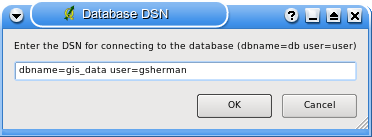
\includegraphics[scale=0.8]{getdsn}
\end{center}
\end{figure}

Para añadir la capa \textsl{world\_borders}, pulse en la herramienta \textsl{Añadir capa} y navegue al 
directorio de datos. Seleccione el archivo shape y pulse \textsl{Abrir} para añadirla al mapa. Se aplicará nuestro 
color personalizado y el resultado es:

\begin{figure}[ht]
\begin{center}
  \caption{Añadir una capa a la aplicación de demostración}\label{fig:demo_app_done}\smallskip
  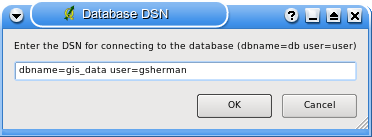
\includegraphics[scale=0.8]{getdsn}
\end{center}
\end{figure}

Crear una aplicación de PyQGIS es realmente muy sencillo. En menos de 150 líneas de código tenemos una aplicación que 
puede cargar una archivo shape y navegar por el mapa. Si juega un poco con el mapa, notará que algunas de las 
funciones incrustadas del lienzo también funcionan, incluido el desplazamiento con la rueda del ratón y la 
panorámica manteniendo pulsada la barra \textsl{Espacio} y moviendo el ratón.

Algunas aplicaciones sofisticadas se han creado usando PyQGIS y más están en camino. Esto es bastante impresionante, 
considerando que este desarrollo ha tenido lugar incluso antes del lanzamiento oficial de QGIS 0.9.

\begin{Tip}\caption{\textsc{Documentación para PyQGIS}}
\qgistip{Tanto si está escribiendo un complemento o una aplicación en PyQGIS, va a necesitar consultar tanto la 
documentación de la API de QGIS (\url{http://qgis.org}) como la Guía de referencia de enlaces Python PyQt 
(PyQt Python Bindings Reference Guide)
(\url{http://www.riverbankcomputing.com/Docs/PyQt4/pyqt4ref.html}). 
Estos documentos proporcionan información sobre las clases y métodos que usará para dar vida a su creación de 
Python.
}
\end{Tip} 